%%%%%%%%%%%%%%%%%%%% author.tex %%%%%%%%%%%%%%%%%%%%%%%%%%%%%%%%%%%
%
% sample root file for your "contribution" to a contributed volume
%
% Use this file as a template for your own input.
%
%%%%%%%%%%%%%%%% Springer %%%%%%%%%%%%%%%%%%%%%%%%%%%%%%%%%%


% RECOMMENDED %%%%%%%%%%%%%%%%%%%%%%%%%%%%%%%%%%%%%%%%%%%%%%%%%%%
\documentclass[graybox]{svmult}

% choose options for [] as required from the list
% in the Reference Guide

%\usepackage{mathptmx}       % selects Times Roman as basic font

\usepackage{helvet}         % selects Helvetica as sans-serif font
\usepackage{courier}        % selects Courier as typewriter font
\usepackage{type1cm}        % activate if the above 3 fonts are
                            % not available on your system
%
\usepackage{makeidx}         % allows index generation
\usepackage{graphicx}        % standard LaTeX graphics tool
                             % when including figure files
\usepackage{multicol}        % used for the two-column index
\usepackage[bottom]{footmisc}% places footnotes at page bottom

% see the list of further useful packages
% in the Reference Guide

\usepackage[T1]{fontenc}
\usepackage{ae,aecompl}
\usepackage{caption}
\usepackage{subcaption}
\captionsetup{compatibility=false}

\usepackage{float}
\floatstyle{plaintop}
\restylefloat{table}

\usepackage{xspace} % for CS macro

\usepackage{xr} % for cross references between different .tex files
\externaldocument{abstract}
\externaldocument{introduction}
\externaldocument{related_work}
\externaldocument{code_saturne}
\externaldocument{using_catalyst}
\externaldocument{results}
\externaldocument{conclusion}

\widowpenalty=10000
\clubpenalty=10000
\setlength{\belowcaptionskip}{+0.3ex}
\setlength{\abovecaptionskip}{3pt plus 3pt minus 2pt}

\makeindex             % used for the subject index
                       % please use the style svind.ist with
                       % your makeindex program

%%%%%%%%%%%%%%%%%%%%%%%%%%%%%%%%%%%%%%%%%%%%%%%%%%%%%%%%%%%%%%%%%%%%%%%%%%%%%%%%%%%%%%%%%

\newcommand{\CS}{%
  {\fontfamily{ppl}\fontshape{it}\selectfont Code\_Saturne}\xspace}

%%%%%%%%%%%%%%%%%%%%%%%%%%%%%%%%%%%%%%%%%%%%%%%%%%%%%%%%%%%%%%%%%%%%%%%%%%%%%%%%%%%%%%%%%

\begin{document}

\title*{In-Situ Visualization in Fluid Mechanics using Open-Source tools: integration of Catalyst into \CS}
% Use \titlerunning{Short Title} for an abbreviated version of
% your contribution title if the original one is too long
\author{Name of First Author and Name of Second Author}
% Use \authorrunning{Short Title} for an abbreviated version of
% your contribution title if the original one is too long
\institute{Name of First Author \at Name, Address of Institute, \email{name@email.address}
\and Name of Second Author \at Name, Address of Institute \email{name@email.address}}
%
% Use the package "url.sty" to avoid
% problems with special characters
% used in your e-mail or web address
%
\maketitle

\abstract{
The volume of data produced by numerical simulations performed on high
performance computers is becoming increasingly large. The visualization of these
large post-generated volumes of data is currently a bottleneck for the
realization of engineering and physics studies in industrial environments. In
this context, Catalyst is a prototype in-situ visualization library developed by
Kitware to help reduce the data post-treatment overhead. On the other side, 
\CS is a Computational Fluid Dynamics code used at EDF, one of the biggest
electricity producers in Europe, for its large scale simulations. In this
chapter we present a study case where Catalyst is integrated into \CS.
We evaluate the feasibility and performance of this integration by running
several use cases in one of our corporate supercomputers.
} % end of abstract


\section{Introduction}
Computational Fluid Dynamics (CFD) is a fundamental step for the study and
optimization of electricity production. Indeed, current power plants use water
as a mean of convective heat transfer. Consequently, the simulation and
visualization of fluid dynamics phenomena is of great importance for the energy
industry. Electricité de France (EDF), one of the largest electricity producer in Europe, has
been developing for the past 15 years an open source CFD code named \CS. \CS performs
CFD computations on very large models~\cite{5644955}. EDF owns
several supercomputers that regularly run this code in order to perform CFD
analysis involving large amounts of data. In this context, the post-processing
and visualization steps become critical. 
%% =======

EDF also develops, in collaboration with OpenCascade and the French Center of
Atomic Research (CEA), an open-source numerical simulation platform called
SALOME~\cite{4291178}. This platform provides generic methods for pre- and post-processing of
numerical simulations. SALOME is based on an open architecture made of reusable
components such as computer-aided design (CAD),
meshing, high performance computing (HPC) execution management, multi-physics coupling, data post-processing
and visualization. The visualization module of the SALOME platform is currently based
on the open-source post-processing platform ParaView. Furthermore, \CS is often used 
in conjunction with the SALOME platform.

In the past, studies and improvements in scientific simulation have been mainly
focused on the solver, due to being the most cycle-consuming part in the
simulation process. Thus, visualization has been traditionally run sequentially
on a smaller computer and at the very end of the solver computation. At the
time, this was easily explained by the small need for both memory and
computation resources in most of the visualization cases. Nevertheless, with the
increase of our computational capabilities, we tend to use and generate much
more data than what we were used to. Thus, as the scale of CFD simulation
problems is getting wider, specific issues are emerging related to input/output
efficiency. In particular, data generated during the solver computation and
used for the visualization are the source of a worrisome overhead. Even worse,
some researchers are starting to spend more time writing and reading data
than actually running solvers and visualizations~\cite{1742-6596-125-1-012099}.
%Sometimes referred as Big Data, 
This new trend compels us to design new input/output (I/O) strategies and consider
visualization as a part of our high-performance simulation systems.

For some years, $in$-$situ$ visualisation techniques have been successfully 
applied in different contexts and mainly by research institutes. 
In this chapter, we present an overview of the efforts 
needed to transition a traditional simulation code to an $in$-$situ$ model 
in an industrial environment. This is the reason why care have been taken 
constructing uses cases that are representative of our current visualisation problems. 

Most fluid dynamic engineers at EDF R\&D are currently visualizing lower temporal and spatial 
resolution versions of their simulations in order to avoid I/O bottlenecks when large quantities of data are involved.
We decided to address the subject of co-processing and $in$-$situ$
visualization which has been proved to be an effective solution against the current
limitations of this problem~\cite{sandiareport}, \cite{4090186}. Our aim is to provide 
EDF engineers with an operational research-oriented tool in a mid-term basis.
%Moreover, while visualization has been traditionnally performed on smaller
%computer, studies show that visualization algorithms can often be run
%efficiently on recent supercomputers~\cite{4090186}. 
For this, we chose to evaluate Catalyst as an industrial tool for performing
$in$-$situ$ visualization. 
Catalyst is a library, developed by Kitware, which implements the
co-processing for ParaView by defining the visualization process through the ParaView user 
interface and exploiting VTK's parallel algorithms for the post-processing of data 
generated by numerical simulation~\cite{6092322}. 

In this chapter, we report a study upon the effectiveness and scalability of a
prototype implementation of the co-processing in an industrial case based on the
coupling of \CS with Catalyst. In section~\ref{sec:motivation} we introduce the motivation of this work.
In section~\ref{sec:related} we
discuss related advances on recent visualization $in$-$situ$ systems. We then
introduce, in section~\ref{sec:cs} \CS, the CFD code developed at EDF
R\&D. In section ~\ref{sec:catalyst} we present our integration of Catalyst into
\CS and how the system is used by EDF users in the context of fluid dynamic
simulations. Section~\ref{sec:results} describes our use case and presents
results on one of our corporate clusters. Finally, section~\ref{sec:conclusion} 
presents our analysis of the results and describes our ongoing and future work.

\section{Related Work}
\label{sec:related}

The size of generated data has become an important subject in high performance 
computing, due to the need of a better I/O efficiency in our computing 
system. To answer this problem, several visualization systems have been created.
We can distinguish two main approaches in recent solutions. The first one is to 
integrate a specific $in$-$situ$ visualization directly to the simulation code. 
Such approach proved to be an efficient way to provide co-processing for a given
simulation as well as a visualization system as it is the case in the hurricane
prediction~\cite{4015457} and earthquake simulation~\cite{4090186} systems.
This method has been proven to lead to good performances but is limited 
to a specific implementation, which does not apply directly to our needs.

The second approach is to provide a general post-processing framework letting the
simulation and the visualization code communicate together. EPSN which is a
general coupling system, allows for the connection of M simulation nodes to N
visualization nodes through a network~\cite{4020782}. This solution is a
loosely coupled approach, requiring separate resources and data transfer
through the network. This approach presents the advantage of not overloading
the nodes used for computation. Thus the visualization code does not interfere
with the execution of the simulation. Based on the same approach, a ParaView
plug-in named ICARUS~\cite{6152102} has been developed. 
It differs from EPSN in design by having lower requirements as it only needs
the use of a single HDF5 library and file driver extension. Such solutions
offer tools for researchers to interact with their simulations by allowing
them, not only to monitor their current states but also to modify
the parameters of the remaining simulation steps. Those computational steering
solutions as well as the RealityGrid
project~\cite{Harting03computationalsteering} focus on interactivity with
simulation whereas our main objective is to provide $in$-$situ$ visualization
operations to researchers while minimizing I/O overhead and disk
space use. 

Both built upon the well known parallel visualization library VTK, 
the application frameworks VisIt~\cite{1532795} and ParaView~\cite{964413} both provide through
the possibility to co-process simulation data via libsim~\cite{2386230} and Catalyst~\cite{6092322} respectively.  
Those $in$-$situ$ solutions are tightly coupled and while they
limit potential interactions with the running simulation, they also highly
reduce the need of network data transfer. Thus, they contribute to circumventing
the inefficiency of high performance computing I/O systems.
Those solutions take their benefits from directly accessing the simulation memory to
perform visualization tasks by simply asking for a pointer to the available
data. One major drawback of this approach is the necessity to provide a coherent data 
layout to those libraries. Moreover, as this type of
solution often gains from computing pre-determined visualization tasks, it is
not well suited for results exploration.  As building a steering solution for Code\_Saturne is out of
the scope of this case study, we do not consider these drawbacks as a limitation. 

After evaluating the performance solutions offered by ParaView and VTK, we choose Catalyst as 
our co-processing library for our case study as it answers EDF's visualization 
needs while focusing on the  reduce of data amount use. Further, Kitware is still actively developing 
Catalyst, and we are optimistic that more services allowing the interactions
with the running simulation will soon be available.


\section{Code\_Saturne: A Computational Fluid Dynamics code}
\label{sec:cs}
Code\_Saturne is an open source computational fluid dynamics software designed
to solve the Navier-Stokes equations in the cases of 2D, 2D axisymmetric or 3D
flows. Its main module is designed for the simulation of flows which may be
steady or unsteady, laminar or turbulent, incompressible or potentially
dilatable, isothermal or not. Scalars and turbulent fluctuations of scalars can
be taken into account. The code includes specific modules, referred to as
“specific physics”, for the treatment of lagrangian particle tracking,
semi-transparent radiative transfer, gas combustion, pulverised coal
combustion, electricity effects (Joule effect and electric arcs) and
compressible flows. Code\_Saturne relies on a finite volume discretisation and
allows the use of various mesh types which may be hybrid (containing several
kinds of elements) and may have structural non-conformities (hanging nodes).The
parallelization is based on standard spatial decomposition with ghost cells
that facilitate data passing between adjacent cells lying across the boundaries
of disconnected decomposed parts using the Message Passing Interface. More
technical details are presented in~\cite{cs2004} and ~\cite{userguide}.


\section{Using Catalyst}
\label{sec:catalyst}
Catalyst is the general purpose coprocessing library of ParaView. This means
that it was designed to work with any simulation code. This behavior is
possible thanks to the use of an adaptor-based architecture. The adaptor binds
the simulation code and Catalyst; it can access both the functions of the
simulation code and the general-purpose API of Catalyst. As Catalyst itself is
independent of the simulation code it is only the adaptor that should be
implemented by the designers of the solver. In our case, we have developed a specific adaptor for
Code\_Saturne. Further explanations on the Catalyst design can be found in
~\cite{6092322}.
All our tests were run on “ParaView 3.98.0 enhanced” and “ParaView 3.98.1”. 

\subsection{Implementing the adaptor}

We identified two main issues to implement our adaptor, the memory management and the handling of ghost cell informations. 

\subsubsection{Memory management}
In order to coprocess the simulation data, Catalyst must be provided with the
data formatted to the VTK data object structure. To accomplish this, several
solutions are possible, essentially depending on the format used for the data
of the simulation code. In the case when the format of the simulation code is
similar to VTK  and, moreover, the simulation data can be shared at any time,
then it is possible to feed Catalyst with a direct pointer to the simulation
memory. Another option is to fully or partially copy the data from the
simulation into a VTK object, and to send this object to Catalyst.

As we provide users of Code\_Saturne with several output formats and as our data
structure in the simulation differs from the VTK data object structure, feeding
Catalyst with a direct pointer to the simulation memory is not possible. Thus,
we chose to copy data from the simulation into a VTK data object. In fact, we
are allocating vtkDoubleArray to store our data for Catalyst. Furthermore, we
provide a pointer of those vtkDoubleArray to Code\_Saturne so it can transform
its simulation data and then fill the VTK data object.

The memory cost increase of our solution can be  alleviated by using more
machines. The cpu cost of the copy is in a range similar to the one needed when
adapting simulation data to a specific output format. This cost is largely
affordable comparatively to the time to write data to disk when storing time
step specific outputs. 

We are currently working on the evolution of our solution. Indeed Kitware plans to
add specific $in$-$situ$ data structures to VTK. This will offer adaptor
developers facilities to make VTK access non VTK compatible simulation data. 

\subsubsection{Handling ghost cells: the vtkDistributedDataFilter}
Handling ghost cell informations is also an important issue for us. Indeed,
several Code\_Saturne features and visualization filters in ParaView rely on the
use of ghost data. Thus allowing the Code\_Saturne and ParaView users to access
this feature is an important objective in our industrial environment.

To address this need, we first tried to rely on the setting of nodes GlobalIds
in order to see if ghost data exchanges between neighbors were already handled
by Catalyst. Indeed ParaView implements a global numbering strategy on its
nodes by using the so-called “GlobalIds”.  While the setting of these GlobalIds
is relevant for the handling of ghost cell informations in ParaView, Catalyst
does not actually use them. As we want Code\_Saturne users to be able to use the
larger scale of both simulation and visualization algorithms, we decided to
force the application of the vtkDistributedDataFilter (D3) filter in the
visualization pipeline. This D3 filter originally performs a redistribution of
the data among the MPI processes but we use it to manage the ghost cells. 

\subsection{Pipeline Configuration Tools}
\label{sec:pip_conf_tools}
From the point of view of an engineer performing a fluid mechanics simulation
using Code\_Saturne, the workflow of a coprocessing-simulation is: 1) to define
a ParaView pipeline describing what the user wants to study and 2) to run the
simulation. As users are already familiar with how to perform fluid mechanics
simulations, defining the pipeline for the coprocessing will be their main
issue. Thus this new process should be done in an efficient and easy way, at
least this part should not become a cumbersome bottleneck. In our industrial
environment this point is of great importance.

The definition of a Catalyst pipeline is possible in two ways. First, the
pipeline can be defined programatically, a solution that we evaluate as too
complicated and time consuming for the end user, especially when setting camera
parameters is needed. Secondly,  the pipeline can be created using the ParaView
user's interface. This second solution is much easier for the user as he/she
can  simply interact with ParaView in the same way he/she used to when
visualizing the results a posteriori. This last solution is the one we 
opted for and it can
be performed after activating the coprocessing plugin in ParaView. 

However, the chosen strategy for defining the pipeline implies a potential
important bottleneck that we want to discuss in detail. Indeed, how can we a
priori define a pipeline on the large geometry and fields that are going to
be used in the simulation ? This is by itself a challenge and could imply a
dedicated parallel system only to define the pipeline. Our solution consists in
using a simplified or under-sampled version of the large geometry to define the
pipeline. In fact, this strategy is possible in ParaView but some
characteristics of the initial geometry must be present in its simplified version (principally equal
names of fields).

Finally, the workflow of our engineers implies several steps to define the
pipeline.  First of all, the users possess a CAD (Computer Aided Design)
version of the geometry that is parametrized. This parametric representation
can generate meshes at different resolution factors. In our case, this is
performed inside the open-source SALOME~\cite{4291178} platform for numerical simulation. 

We generate two different meshes, one at high resolution (up to 204M
hexahedrals in the use cases of this article) that will be used for the CFD
simulation and one with a lower resolution to define the pipeline (700 000
hexahedrals in our use cases). The lowest resolution mesh is fed into Code\_Saturne to perform a short
simulation. This allows ParaView to obtain a representation containing not
only the geometry but also the result fields. This is the data that is 
actually used to define the pipeline.


\section{Results}
\label{sec:results}

\subsection{Required User Interactions for Co-processing}
   
Before presenting our results we briefly describe how the user interactions were
performed. The following steps were necessary in order to use the developed
co-processing technology:

1) A ``light version'' of the input mesh is generated as explained in section~\ref{sec:pip_conf_tools}. 
As the user possesses a CAD version of the geometry that is parametrized, it is then possible to
obtain meshes at different spatial resolutions. A ``light mesh'' of small size in
memory and representative of the CAD geometry is obtained. Figure~\ref{fig:piece} represents
the ``light version'' of the mesh used in our experiments.

2) A short simulation (normally just a few seconds on a local machine) on the ``light mesh'' is run.
This simulation allows to define the information about the result fields needed to create a
visualisation pipeline in ParaView (e.g. temperature, pressure, velocity). An ``augmented light mesh''
is therefore created.

3) The mesh and the fields obtained at the end of step 2 are then read in ParaView
and the user defines her/his visualisation pipeline. At the end of this step
a simple click in the ParaView interface will create a Python file that
programmatically defines the visualisation operations to be performed
$in$-$situ$.

4) Finally the real simulation is ran using a full resolution size mesh. The
co-processing part of the simulation reads the python script containing the
definition of the visualisation pipeline. This step is expected to be
time-consuming.

\begin{figure}
  \centering
  \begin{subfigure}[b]{0.45\textwidth}
    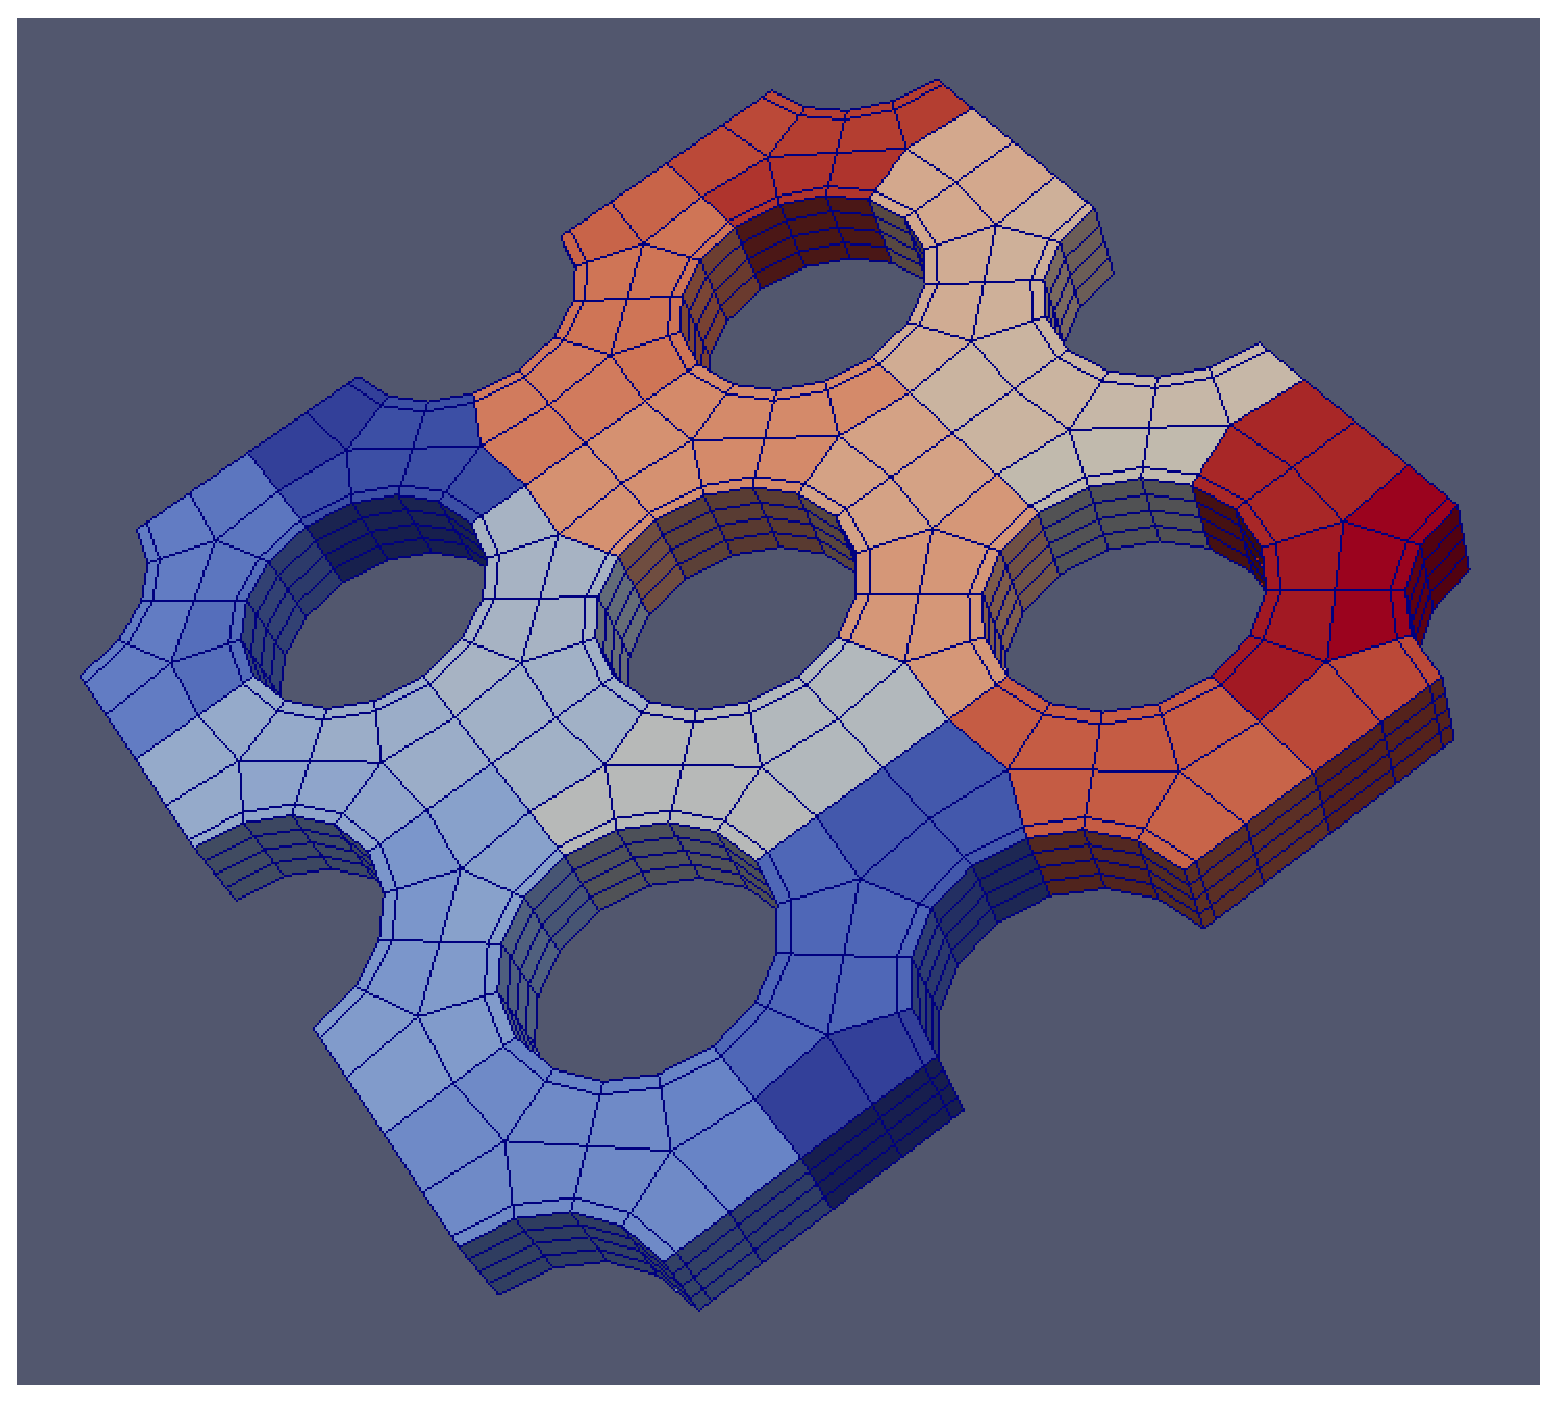
\includegraphics[scale=0.195]{pictures/pieceofcake.eps}
    %\captionof{figure}{Original geometry for our use case}
    \captionof{figure}{}
    \label{fig:piece}
  \end{subfigure}
  ~
  \begin{subfigure}[b]{0.45\textwidth}
    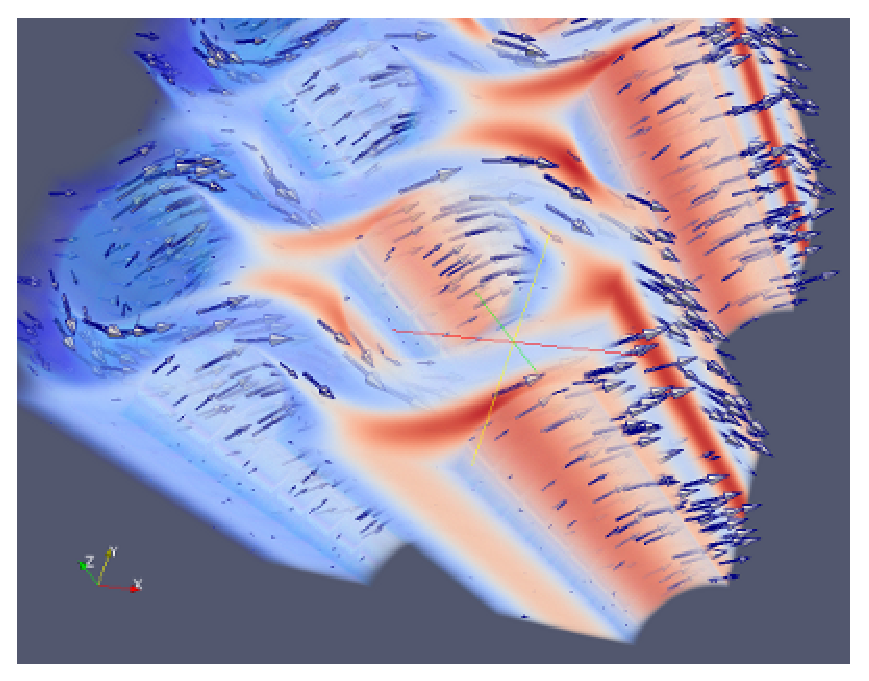
\includegraphics[scale=0.41]{pictures/res.eps}
    %\captionof{figure}{A final coprocessed picture of our simulation. The simulation was run with 128 layers.}
    %\captionof{figure}{A final coprocessed picture of our simulation.}
    \captionof{figure}{}
    \label{fig:res}
  \end{subfigure}
  \caption{(a) original geometry of our use case\\
  \hspace{8em}(b)  a final coprocessed picture of our simulation}
\end{figure}

\subsection{Use Cases}

Our simulations have been run on Ivanoe, an EDF corporate supercomputer,
composed of 1382 nodes, each node having 12 cores for a total of 16584 cores. In
these simulations we associate one MPI process by core and we use from 720 cores up
to 3600 cores. We include two use cases that were run on this supercomputer. The
choice of the cases is motivated by two main factors: the size of the mesh and
the complexity of the visualization pipeline. We detail next these two impacting factors.

1) Mesh size. We chose to use two meshes representing the same geometry but at
different resolutions, one made of 51M hexahedral elements and another of 204M
hexahedrals. In our industrial environment at EDF most simulation engineers use
meshes composed by less than 51M of element, that is why we chose this mesh size to be
representative of the work performed by an average engineer during his work routine.
Furthermore, a 51M elements mesh more than doubles the size used in the results
presented in~\cite{6092322} for the PHASTA adaptor. On the other hand, when research
oriented simulations are performed at EDF, these simulations currently contain around 200M
elements. We choose this size as a typical research oriented or ``heavy mesh'' simulation data.

2) Pipeline complexity. We define two pipelines aimed to be representative of two
different situations: users performing simple and light visualization
operations (e.g. generating slices in a volume) and another using very
time-consuming visualization tasks (e.g. performing volume rendering).

\begin{table}
\centering
\begin{tabular}{|p{1.5cm}|p{3.0cm}|p{2.70cm}|p{1.50cm}|}
\hline
\multicolumn{4}{|c|}{\textbf{USE CASES SUM UP}}\\
\hline
NAME & SIZE & PIPELINE & FIGURES \\
\hline
 %& & & \\
$CASE$\_$A$ & 51M hexahedrals, \newline industrial size case & \textbf{heavy}:
\newline volume rendering, \newline celldatatopointdata \newline and glyphs  &
5a 5c 5e\\
\hline
 %& & & \\
$CASE$\_$B$ & 204M hexahedrals, \newline research size case & \textbf{light}:
\newline 9 slices,\newline celldatatopointdata  & 5b 5d 5f   \\
\hline
\end{tabular}
%\vspace{-0.1in}
\caption{Description of our two use cases.}
\label{fig:tab}
%\end{figure}
\vspace{-0.15in}
\end{table}
In the following we name our uses cases:
$CASE$\_$A$, use case using an average mesh size of 51M hexahedrals and a
visualization pipeline including volume rendering which aims to be very time-consuming.
$CASE$\_$B$, our second use case, contains a light visualization pipeline simply
performing some slices but on a large mesh of 204M hexahedrals.

Table~\ref{fig:tab} summarizes the composition of these use cases. In all our use cases we
run a simulation consisting in a fluid with physical properties identical to
water passing through the mesh. Then the output is generated at each step, for a
total of 10 co-processed visualization images.

%\vspace{-0.10in}
\subsection{Results}

\begin{figure}
        \begin{subfigure}[b]{0.50\textwidth}
                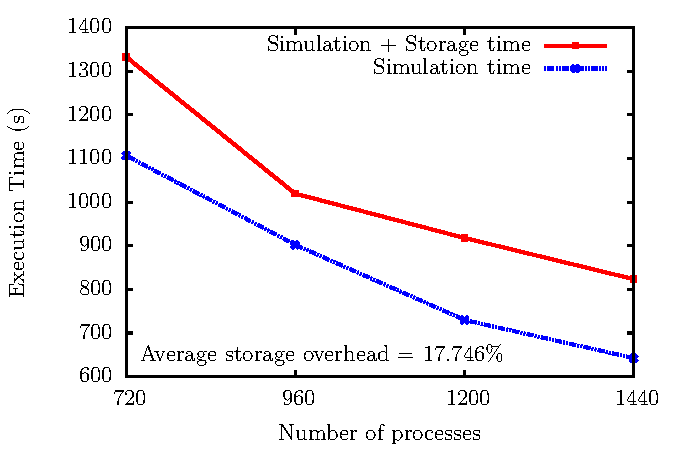
\includegraphics[scale=0.50]{pictures/test41.ps}
                \caption{Time overhead of storage}
                \label{fig:over}
        \end{subfigure}
        ~
        \begin{subfigure}[b]{0.50\textwidth}
                \includegraphics[scale=0.50]{pictures/test42.ps}
                \caption{Time overhead of storage}
                \label{fig:204over}
        \end{subfigure}

        \begin{subfigure}[b]{0.50\textwidth}
          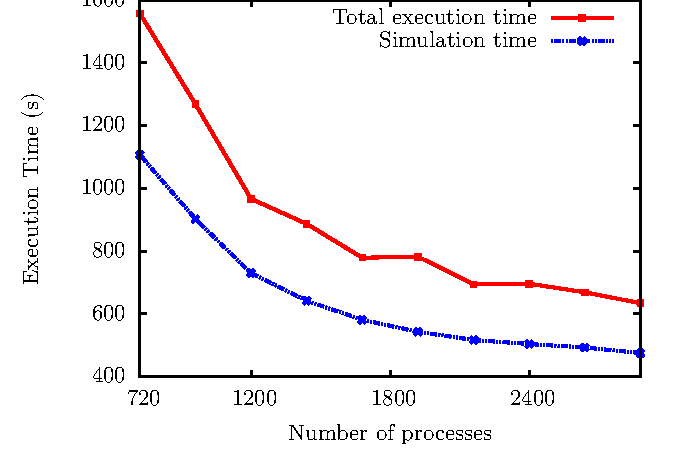
\includegraphics[scale=0.50]{pictures/test1.ps}
                \caption{Execution time with/out coprocessing}
                \label{fig:copro}
        \end{subfigure}%
        ~
        \begin{subfigure}[b]{0.50\textwidth}
          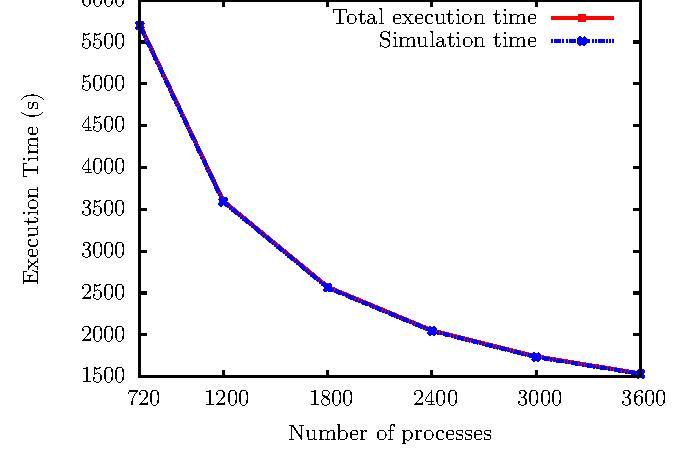
\includegraphics[scale=0.50]{pictures/test12.ps}
                \caption{Execution time with/out coprocessing}
                \label{fig:204copro}
        \end{subfigure}%

        \begin{subfigure}[b]{0.50\textwidth}
                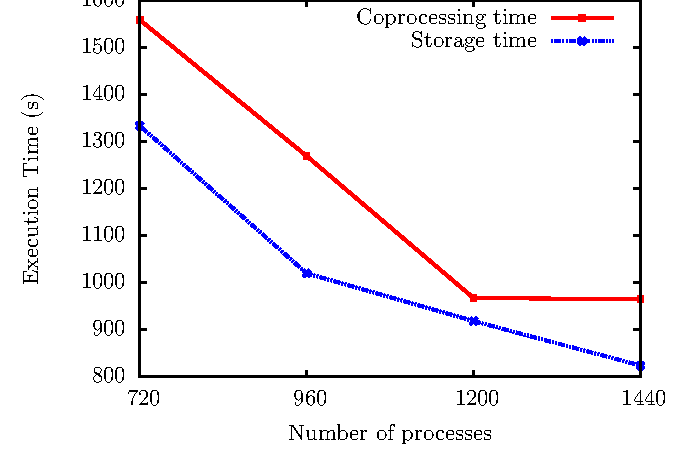
\includegraphics[scale=0.50]{pictures/test2.ps}
                \caption{Execution time comparison with storage.}
                \label{fig:ensight}
        \end{subfigure}
        ~
        \begin{subfigure}[b]{0.50\textwidth}
                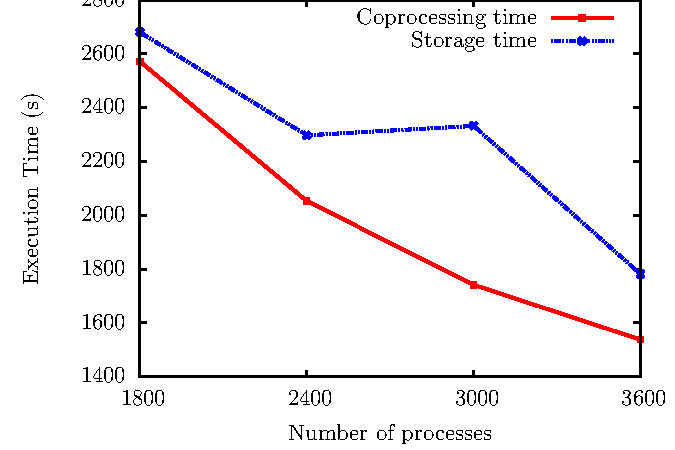
\includegraphics[scale=0.50]{pictures/test22.ps}
                \caption{Execution time comparison with storage.}
                \label{fig:204ensight}
        \end{subfigure}
        \caption{CASE\_A (left) and CASE\_B (right) results}\label{fig:animals}
\end{figure}

Figure~\ref{fig:res} presents an image obtained from one of our $in$-$situ$
simulations with $CASE$\_$A$.
We see the flux of water moving around the vertical cylinders, the glyphs being attached 
to the velocity vectorial field. The color of the volume rendering represents 
the turbulent viscosity of the fluid. 

We establish first the overhead induced by storing our simulation results in
figure~\ref{fig:over} and~\ref{fig:204over}. We observe an average of 18\% and
14\% of time used to store results, for $CASE$\_$A$ and $CASE$\_$B$
respectively. These figures correspond to the comparison of $T_w$ and $T_s +
T_w$ in equation~\ref{eq:first}. 
This overhead tends to increase with the number of processes in
use. One can also notice that the overhead is also not stable and subject 
to important variations with a peak at
26\%. We thus identify the storage process as a bottleneck in everyday CFD
studies for its average overhead and its high instability in execution time.

Figure~\ref{fig:copro} shows two graphs of $CASE$\_$A$: in red the execution 
time versus the number of cores, in blue the execution time without
the co-processing overload. These figures correspond to the comparison of $T_s$
and $T_s + T_{process}$ in equation~\ref{eq:second}.
We are satisfied by this overload that is comprised between 20 and 30\% of the total execution time, 
when we chose complicated task with a high $T_{process}$.
Moreover, it looks like this overload is decreasing when the number of cores increases. 
Figure~\ref{fig:204copro} shows the exact same behavior in the $CASE$\_$B$ experiment. Both
graphs are difficult to distinguish as the time needed for co-processing is
circumscribed between 6 and 10 seconds, the overload (the difference between $T_s$ and $T_s + T_{process}$) is less than one
percent of the total execution time. We notice that having heavy $T_{process}$ is not very usual in our applications and 
we consider $CASE$\_$A$ as an example of worst case scenario.

We also decided to compare the Catalyst overhead with a non-VTK-based 
storage strategy that performs no visualization operations. Figure~\ref{fig:ensight} and~\ref{fig:204ensight}, 
show the comparison of the global execution time with Catalyst co-processing
versus the Ensight Gold storage format. This means comparing $T_s + T_w$ 
and $T_s + T_{process} + T_{w-in-situ}$. Figure~\ref{fig:ensight} presents
our implementation results with $CASE$\_$A$. This compares positively for Catalyst as the overhead
is approximately 10\% and decreases when the number of cores increases. We
notice that for $CASE$\_$A$ the heavy $T_{process}$ is already taken into
account in the $in$-$situ$ curve but $T_r + T_v$ is still not performed for the
traditional visualisation scheme. This means that this result is very positive
and we should not forget that $T_r + T_v$ is very time consuming for this case
(and saturates our scientific PCs at EDF R\&D). 

Figure~\ref{fig:204ensight}
presents our results for $CASE$\_$B$. Here we can see the potential of Catalyst
when 
lighter and more relevant visualization tasks are processed. Indeed, there is no more 
overhead as we gain an average of 10\% of execution time while freeing
ourselves from storage issues (we evaluate the execution time peak of
3000 processes as a result of concurrent accesses on our 
supercomputer storage disks). To emphasize this, Table~\ref{fig:size_tab} shows how much data each
solution generates, namely a basic storage in Ensight Gold format versus our
co-processing implementation using Catalyst. These informations are those of our
CASE\_B when performing a 10 steps simulation. Both size are
expected to grow proportionally to the size of the mesh input, and the number of
steps. Therefore, we expect the gain provided by the use of co-processing 
to be increasingly interesting when moving forward in use case size.

\begin{table}[!h]
\centering
\begin{tabular}{|p{3.5cm}|p{3.5cm}|}
\hline
\multicolumn{2}{|c|}{\textbf{*PROCESSING SIZE COMPARISON}}\\
\hline
STORAGE & COPROCESSING \\
\hline 
 %& \\
57Gio & 1,3Mio \\
\hline 
\end{tabular} 
%\vspace{-0.1in}
\caption{CASE\_B comparison between the size of processed results and simple storage. The simulation was run on 10 steps, with 10
pictures co-processed.}
\label{fig:size_tab}
%\end{figure}
\end{table}


\section{Conclusion}
\label{sec:conclusion}

We have successfully integrated Catalyst into Code\_Saturne (a computational
fluid dynamics code developed at EDF R\&D). After testing the prototype in our
corporate supercomputer Ivanoe, we find Catalyst to be a relevant solution to
provide Code\_Saturne users with visualization coprocessing.  Catalyst proved to allow a
simple and fast implementation of an adaptor. We use D3 (a filter originally 
performing a redistribution of the data among MPI processes) as a ghost cell
handler. We feel that the code responsible for the ghost cells management in D3
could be integrated directly into ParaView/Catalyst since applying D3 can be
time consuming.  

Our preliminary results are based on a 51M and a 204M elements mesh, which is above the
average size case used by EDF engineers in our industrial environment.  We plan
to perform simulation on at least 400M elements meshes in the near future.  
We have also
performed simulation up to 300 nodes and are currently planning not using more
in this cluster. This is due to the typical simulation node size
being around 150 nodes for our engineers.  We also plan to work on another of
our corporate supercomputers, an IBM BG/Q with 65k cores. In that case, we will
test on a much bigger number of cores.  The increase of memory use found in the
results section indicates that memory optimizations are to be performed before
running on the IBM BG/Q. We did not in this study perform any delicate memory
tweaking in order to reduce the memory consumption. We are currently working on
this point, experimenting new VTK $in$-$situ$ data structures that may highly
reduce this overhead.

We are mostly satisfied with the integration of Catalyst in Code\_Saturne.
Our first version of our integration will be most probably released in September 
2013 as part of a new version of this open-source software. 


\input{referenc}
\end{document}
